% ========== HAVLIT ==========
\begin{frame}{%
  \begin{minipage}[t]{0.32\textwidth}
    Havlit
  \end{minipage}%
  \hfill
  \begin{minipage}[t]{0.36\textwidth}
    \centering
    \footnotesize\textbf{Jagttid:} Ingen jagttid
  \end{minipage}%
  \hfill
  \begin{minipage}[t]{0.15\textwidth}
    \noindent\raggedleft
    
\includegraphics[width=0.5cm, height=0.5cm, keepaspectratio]{Billeder/Ikoner/star.png}
  \end{minipage}%
}
  \vspace{0.25em}
  \begin{columns}[T]
    % --- Venstre kolonne: Tekst ---
    \column{0.55\textwidth}
    \setlength{\parskip}{0.5em}
    \tiny
    \RaggedRight
    \textbf{\textit{Clangula hyemalis}} – lille dykand med meget lang hale \par
    \textbf{Udseende:}\\
    \quad – Andrik: Brun, sort, hvid med meget lange halefjer \par
    \quad – And: Hvid, brun spraglet, kort kraftigt næb
    % --- Højre kolonne: Billeder ---
    \column{0.40\textwidth}
    \centering
    \fbox{%
      \begin{minipage}{\linewidth}
        \centering
        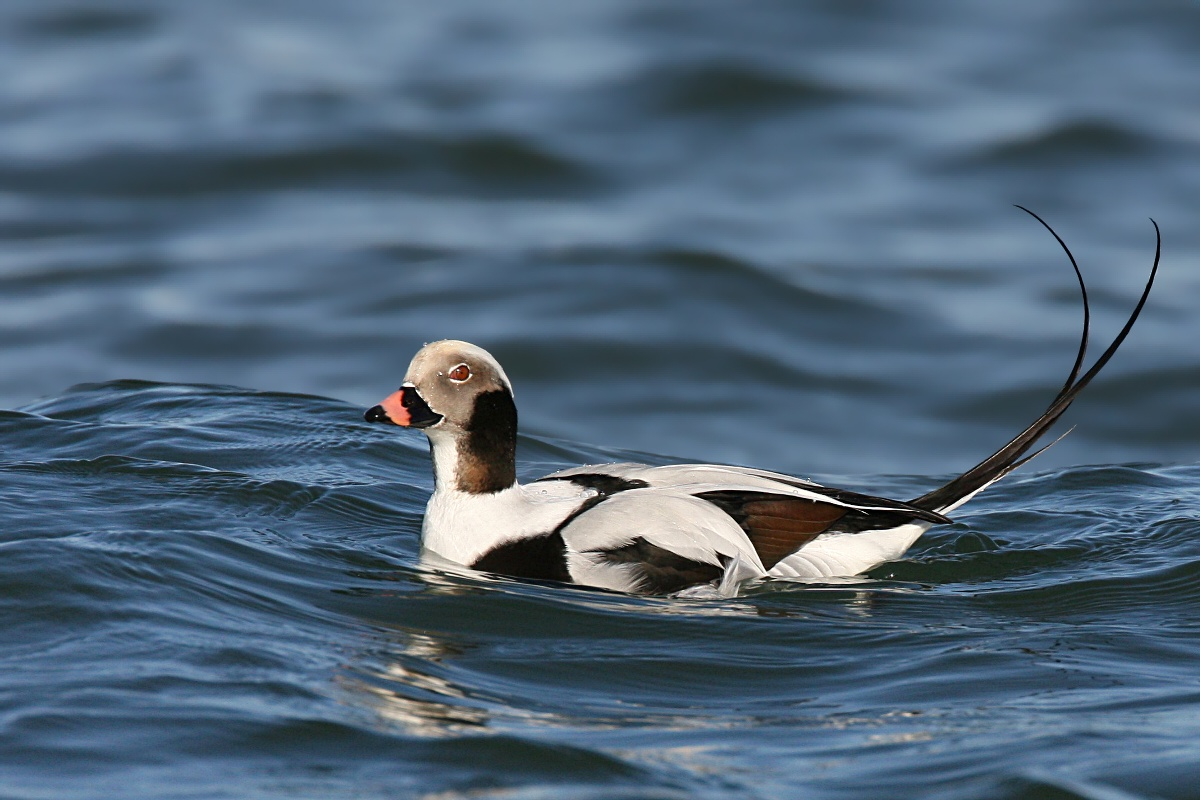
\includegraphics[width=0.7\linewidth, height=3cm, keepaspectratio]{Billeder/Dyr/Fugle/Aender/Dykaender/havlit_han.jpg}\\[0.5em]
        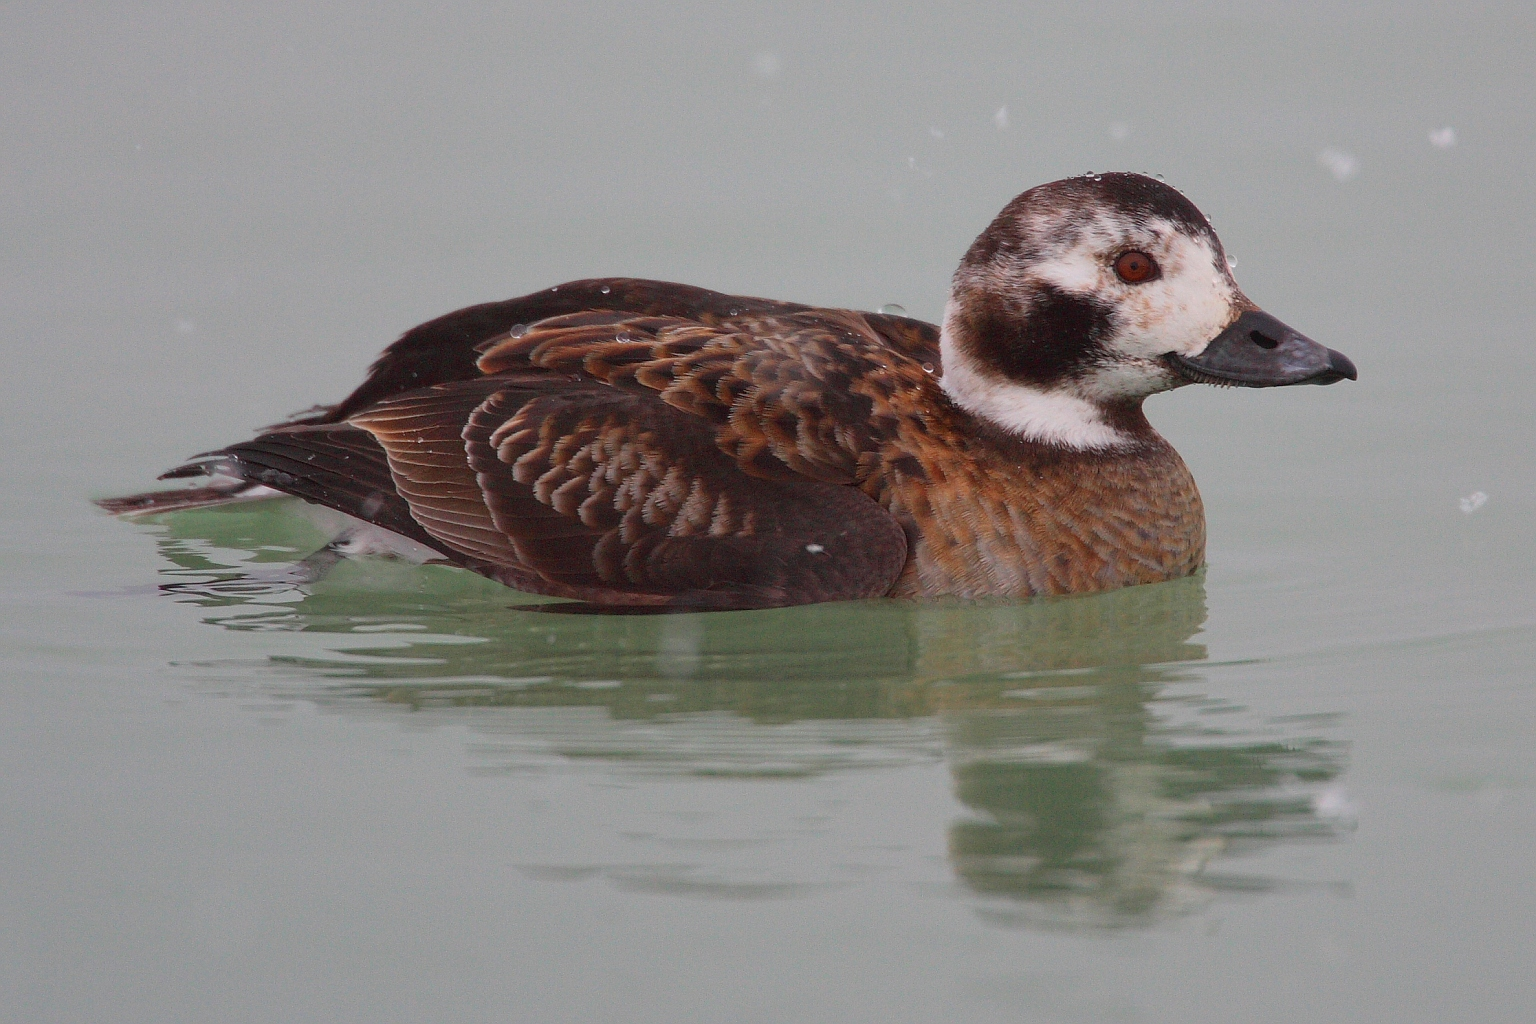
\includegraphics[width=0.7\linewidth, height=3cm, keepaspectratio]{Billeder/Dyr/Fugle/Aender/Dykaender/havlit_hun.jpg}%
      \end{minipage}
    }%
    \vspace{0.05em}
    \footnotesize Andrik øverst, and nederst
  \end{columns}
\end{frame}